\section{Today's assignment}
Today's class will be focused on advanced deep learning concepts, mainly
Recurrent Neural Networks (RNNs). In the first day we saw how the chain-rule
allowed us to compute gradients for arbitrary computation graphs. Today we will
see that we can still do this for more complex models like Recurrent Neural
Networks (RNNs). In these models we will input data in different points of the
graph, which will correspond to different time instants. The key factor to
consider is that, for a fixed number of time steps, this is still a computation
graph and all what we saw on the first day applies with no need for extra math.

If you managed to finish the previous day completely you should aim at finishing
this as well. If you still have pending exercises from the first day e.g. the
Pytorch part. It is recommended that you try to solve them first and then
continue with this day. 

\section{Recurrent Neural Networks: Backpropagation Through Time}

\subsection{Feed Forward Networks Unfolded in Time}

\begin{figure}[!h]
\centering
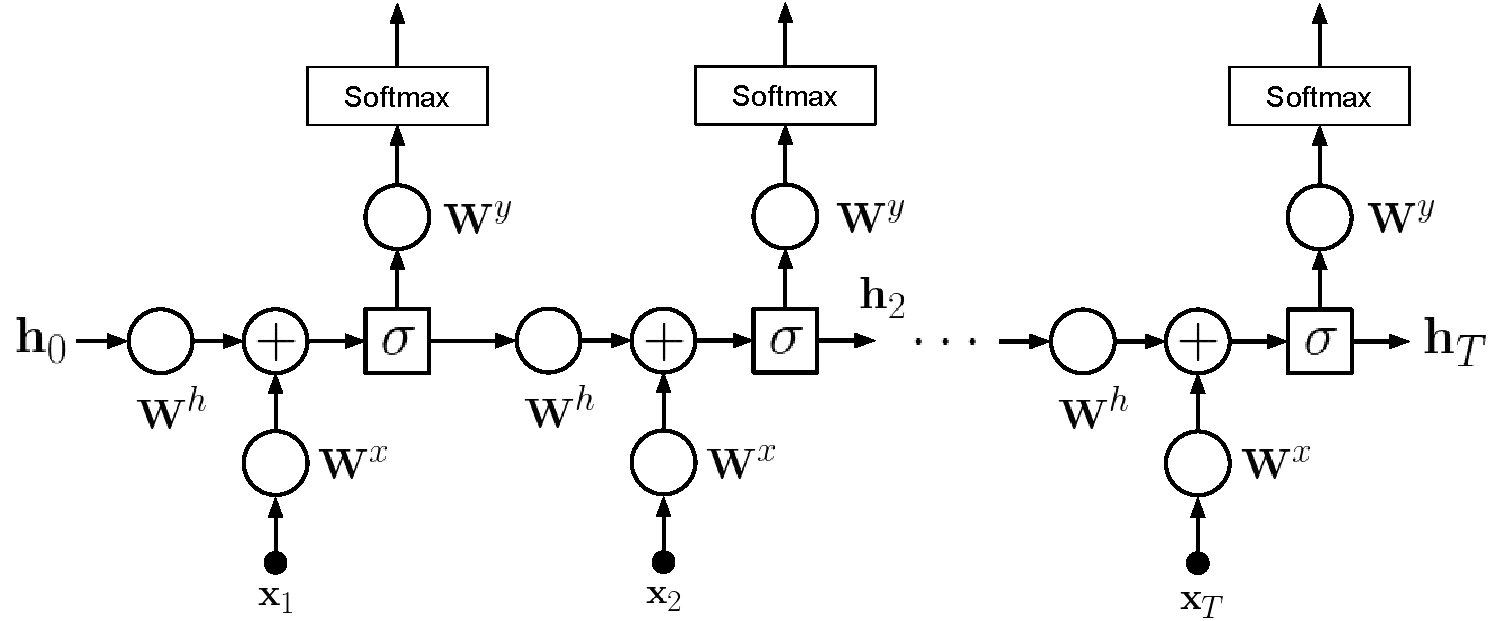
\includegraphics[scale=0.6]{figs/deep_learning/RNN2.pdf}
\caption{The simplest RNN can be seen as replicating a single hidden-layer FF
network $T$ times and passing the intermediate hidden variable $\mathbf{h}_t$
across different steps. Note that all nodes operate over vector inputs e.g,.
$\mathbf{x}_t \in \mathbb{R}^I$. Circles indicate matrix multiplications.}
\label{fig:RNN}
\end{figure}

We have seen already Feed Forward (FF) networks. These networks are ill
suited to learn variable length patterns since they only accept inputs of a
fixed size. In order to learn sequences using neural networks, we need therefore
to define some architecture that is able to process variable length inputs.
Recurrent Neural Networks (RNNs) solve this problem by unfolding the
computation graph in time. In other words, the network is replicated as many
times as it is necessary to cover the sequence to be modeled. In order
to model the sequence one or more connections across different time instants are
created. This allows the network to have a memory in time and thus capture
complex patterns in sequences. In the simplest model, depicted in
Fig.~\ref{fig:RNN}, and detailed in Algorithm~\ref{algo:rnnforward}, a RNN is
created by replicating a single hidden-layer FF network $T$ times and passing
the intermediate hidden variable across different steps. The strength of the
connection is determined by the weight matrix $\mathbf{W}_h$

\subsection{Backpropagating through Unfolded Networks}

\begin{figure}[!h]
\centering
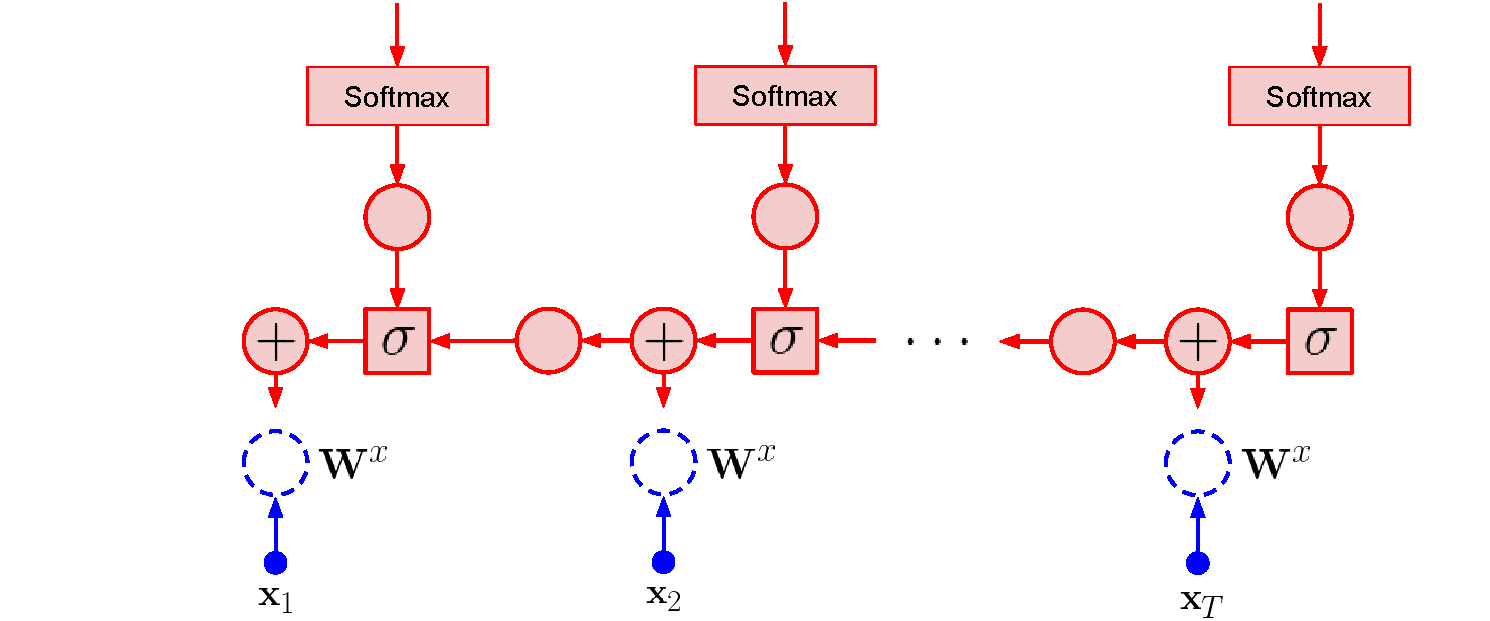
\includegraphics[scale=0.6]{figs/deep_learning/RNN2_backprop.pdf}
        \caption{Forward-pass (blue) and backpropagated error (red) to the input layer of an RNN. Note that a copy of the error is sent to each output of each sum node $(+)$}
\label{fig:RNN}
\end{figure}

It is important to note that there is no formal changes needed to apply
backpropagation to RNNs. It concerns applying the chain rule just as it
happened with FFs. It is however useful to consider the following properties of
derivatives, which are not relevant when dealing with FFs

\begin{itemize}
\item When two variables are summed up in the forward-pass, the error is backpropagated to each of the summand sub-graphs
\item When unfolding in $T$ steps the same parameters will be copied $T$ times. All updates for each copy are summed up to compute the total gradient. 
\end{itemize}

Despite the lack of formal changes, the fact that we backpropagate an error
over the length of the entire sequence often leads to numerical problems. The
problem of \textit{vanishing} and \textit{exploding} gradients are a well know
limitation. A number of solutions are used to mitigate this issue. One simple,
yet inelegant, method is clipping the gradients to a fixed threshold. Another
solution is to resort to more complex RNN models that are able to better handle
long range dependencies and are less sensitive to this phenomena. It is
important to bear in mind, however, that all RNNs still use backpropagation as
seen in the previous day, although it is often referred as
\textit{Backpropagation through time}. 

\begin{algorithm}[th!]
\label{algo:rnnforward}
   \caption{Forward pass of a Recurrent Neural Network (RNN)}
\begin{algorithmic}[1]

   \STATE {\bfseries input:} Initial parameters for an RNN Input
$\Theta=\{\mathbf{W}^x \in \mathbb{R}^{H \times I}, \mathbf{W}^h \in \mathbb{R}^{H \times H}, \mathbf{W}^y \in \mathbb{R}^{K \times H} \}$ input, recurrent and output transformations respectively.

   \STATE {\bfseries input:} Input data matrix $\mathbf{x} \in \mathbb{R}^{I \times T}$ of size $T$. Initial recurrent variable $\mathbf{h}_0$. 

	\FOR{$t=1$ {\bfseries to} $T-1$}
     \STATE Apply linear transformation combining input and recurrent signals
        $$z_{jt}^h = \sum_{i=1}^{I} W_{ji}^x x_{it} + \sum_{j'=1}^{J} W_{jj'}^h h_{j't-1}$$
     \STATE Apply non-linear transformation e.g. sigmoid (hereby denoted $\sigma()$)
     $$h_{jt} = \sigma(z_{jt}^h)  = \frac{1}{1+\exp(-z_{jt}^h)}$$

	\ENDFOR

\STATE Apply final linear transformation to each of the recurrent variables $\mathbf{h}_1 \cdots \mathbf{h}_T$ 
   $$z_{kt}^y = \sum_{j=1}^{J} W_{kj}^y h_{jt}$$
\STATE Apply final non-linear transformation e.g. softmax 
$$p(y_t=k|\mathbf{x}_{t:}) = \frac{\exp(z_{kt}^y)}{\sum_{k'=1}^{K} \exp(z_{k't}^y)}$$

\end{algorithmic}
\end{algorithm}


\begin{exercise}
\label{exercise:rnnnumpy}
Convince yourself that a RNN is just an FF unfolded in time. Complete the 
backpropagation() method in NumpyRNN class in lxmls.deep\_learning\_numpy\_models.rnn.py
and compare it with\\ lxmls.deep\_learning\_numpy\_models.mlp.py.\\

\noindent To work with RNNs we will use the Part-of-speech data-set seen in the
sequence models day.
\begin{python}
# Load Part-of-Speech data 
from lxmls.readers.pos_corpus import PostagCorpusData
data = PostagCorpusData() 
\end{python}
\clearpage
\noindent Load and configure the NumpyRNN. Remember to use reload if you want to modify 
the code inside the rnns module
\begin{python}
# Instantiate RNN
from lxmls.deep_learning.numpy_models.rnn import NumpyRNN
model = NumpyRNN(
    input_size=data.input_size,
    embedding_size=50,
    hidden_size=20,
    output_size=data.output_size,
    learning_rate=0.1
)
\end{python}
As in the case of the feed-forward networks you can use the following setup to
test step by step the implementation of the gradients. First compute the cost
variation for the variation of a single weight
\begin{python}
from lxmls.deep_learning.rnn import get_rnn_parameter_handlers, get_rnn_loss_range

# Get functions to get and set values of a particular weight of the model
get_parameter, set_parameter = get_rnn_parameter_handlers(
    layer_index=-1,
    row=0, 
    column=0
)

# Get batch of data
batch = data.batches('train', batch_size=1)[0]

# Get loss and weight value
current_loss = model.cross_entropy_loss(batch['input'], batch['output'])
current_weight = get_parameter(model.parameters)

# Get range of values of the weight and loss around current parameters values
weight_range, loss_range = get_rnn_loss_range(model, get_parameter, set_parameter, batch)
\end{python}
then conmpute the desired gradient from your implementation
\begin{python}
# Get the gradient value for that weight
gradients = model.backpropagation(batch['input'], batch['output'])
current_gradient = get_parameter(gradients)
\end{python}
and finally call matlplotlib to plot the loss variation versus the gradient
\begin{python}
%matplotlib inline
import matplotlib.pyplot as plt
# Plot empirical
plt.plot(weight_range, loss_range)
plt.plot(current_weight, current_loss, 'xr')
plt.ylabel('loss value')
plt.xlabel('weight value')
# Plot real
h = plt.plot(
    weight_range,
    current_gradient*(weight_range - current_weight) + current_loss, 
    'r--'
)
\end{python}
\clearpage
After you have completed the gradients you can run the model in the POS task
\begin{python}
import numpy as np
import time

# Hyper-parameters
num_epochs = 20

# Get batch iterators for train and test
train_batches = data.batches('train', batch_size=1)
dev_set = data.batches('dev', batch_size=1)
test_set = data.batches('test', batch_size=1)

# Epoch loop
start = time.time()
for epoch in range(num_epochs):

    # Batch loop
    for batch in train_batches:
        model.update(input=batch['input'], output=batch['output'])

    # Evaluation dev
    is_hit = []
    for batch in dev_set:
        is_hit.extend(model.predict(input=batch['input']) == batch['output'])
    accuracy = 100*np.mean(is_hit)
    print("Epoch %d: dev accuracy %2.2f %%" % (epoch+1, accuracy))

print("Training took %2.2f seconds per epoch" % ((time.time() - start)/num_epochs))

# Evaluation test
is_hit = []
for batch in test_set:
    is_hit.extend(model.predict(input=batch['input']) == batch['output'])
accuracy = 100*np.mean(is_hit)

# Inform user
print("Test accuracy %2.2f %%" % accuracy)
\end{python}
\end{exercise}

\clearpage
\section{Implementing your own RNN in Pytorch}

One of the big advantages toolkits like Pytorch or Dynet is that creating computation graphs that dynamically change size is very simple. In many other tookits it is directly not possible to use a Python for loop with a variable length to define a computation graph. Again, as in other toolkits we will only need to create the forward pass of the RNN and the gradients will be computed automatically for us.

\begin{exercise}
As we did with the feed-forward network, we will no implement a
Recurrent Neural Network (RNN) in Pytorch. For this complete the
log\_forward() method in lxmls/deep\_learning/pytorch\_models/rnn.py.

\noindent Load the RNN model in numpy and Python for comparison
\begin{python}
# Numpy version
from lxmls.deep_learning.numpy_models.rnn import NumpyRNN
numpy_model = NumpyRNN(
    input_size=data.input_size,
    embedding_size=50,
    hidden_size=20,
    output_size=data.output_size,
    learning_rate=0.1
)

# Pytorch version
from lxmls.deep_learning.pytorch_models.rnn import PytorchRNN
model = PytorchRNN(
    input_size=data.input_size,
    embedding_size=embedding_size,
    hidden_size=hidden_size,
    output_size=data.output_size,
    learning_rate=learning_rate
)
\end{python}
\noindent To debug your code you can compare the numpy and Pytorch gradients using
\begin{python}
# Get gradients for both models
batch = data.batches('train', batch_size=1)[0]
gradient_numpy = numpy_model.backpropagation(batch['input'], batch['output'])
gradient = model.backpropagation(batch['input'], batch['output'])
\end{python}
\noindent and then plotting them with matplotlib
\begin{python}
%matplotlib inline
import matplotlib.pyplot as plt
# Gradient for  word embeddings in the example
plt.subplot(2,2,1)
plt.imshow(gradient_numpy[0][batch['input'], :], aspect='auto', interpolation='nearest')
plt.colorbar()
plt.subplot(2,2,2)
plt.imshow(gradient[0].numpy()[batch['input'], :], aspect='auto', interpolation='nearest')
plt.colorbar()
# Gradient for  word embeddings in the example
plt.subplot(2,2,3)
plt.imshow(gradient_numpy[1], aspect='auto', interpolation='nearest')
plt.colorbar()
plt.subplot(2,2,4)
plt.imshow(gradient[1].numpy(), aspect='auto', interpolation='nearest')
plt.colorbar()
plt.show()
\end{python}
Once you are confident that your implementation is working correctly you can run it on the POS task using the Pytorch code from the Exercise~\ref{exercise:rnnnumpy}. 
\end{exercise}

%\section{Low Level RNN Implementations}
%In the last exercise, you might have notticed that the speed of Pytorch is not bigger than that of numpy. This is due to various reasons including small model size and lack of GPU but also the fact that dynamic for loops are not particularly fast. When there is no need for custom implementations Pytorch has very fast low-level implementations of multiple network topologies. 
%\begin{exercise}
%Instantiate the fast RNN model
%\begin{python}
%\end{python}
%\end{exercise}

%\section{The Importance of Pre-training}
%
%One of the key insights that has played a role in the rise of deep learning in
%NLP tasks is the use of neural word-embeddings. These are just numeric 
%representations of words that can be learned from unsupervised data using
%simple FF networks such as e.g. skip-grams.
%
%Such representations can be plugged into supervised models such as the RNN that we just
%trained to initialize its initial layer. The use of pre-trained embeddings very often leads to
%important improvements in performance. 
%
%\begin{exercise}
%Test the effect of using pre-trained embeddings. Run the following code to
%download the embeddings. Reset the layer parameters and initialize the
%embedding layer with the pre-trained embeddings. Then run the training code
%from the last exercise.
%\begin{python}
%# Embeddings Path
%import lxmls.deep_learning.embeddings as emb
%import os
%reload(emb)
%if not os.path.isfile("data/senna_50"):
%    emb.download_embeddings('senna_50', "data/senna_50")
%E = emb.extract_embeddings("data/senna_50", train_seq.x_dict) 
%# Reset model to remove the effect of training
%rnn = rnns.reset_model(rnn, seed=SEED)
%# Set the embedding layer to the pre-trained values
%rnn.param[0].set_value(E.astype(theano.config.floatX)) 
%
%# Now re-run SGD training
%\end{python}
%\end{exercise}
